% compile using latex (xelatex seems to crop the figure strangley)
\documentclass{article} % For LaTeX2e
\usepackage[dvips]{graphicx}
\usepackage{nips14submit_e,times}
\usepackage{hyperref}
\usepackage{wrapfig}
\usepackage{rotating}
\usepackage[outdir=./]{epstopdf}

\usepackage{graphics,graphicx}
\usepackage{amsmath,amssymb,amsfonts,comment}
\definecolor{LinkColor}{rgb}{0,0,0}    

\newcommand{\p}{\text{P}}
\newcommand{\word}[1]{\texttt{#1}}
\urldef{\googlegroup}\url{https://groups.google.com/forum/#\!forum/word2vec-toolkit}
\urldef{\blogpost}\url{https://blog.lateral.io/2015/06/the-unknown-perils-of-mining-wikipedia/ }

\title{Corpus Experiments for Word Embeddings}

 \author{
 	Benjamin Wilson\\
	Lateral GmbH\\
	\texttt{benjamin@lateral.io}
	\And
	Adriaan Schakel\\
	\texttt{adriaan.schakel@gmail.com}
 }

\date{\today}
\nipsfinalcopy % Uncomment for camera-ready version

\begin{document}

\graphicspath{{../outputs/}}
\maketitle


\begin{abstract}
	We introduce an experimental approach to studying the properties of word embeddings.
	Controlled experiments, acheived by modification of the training corpus, permit the demonstration of direct, causal relationships between word properties and word vector direction and length.
	This approach is demonstrated in the case of the word2vec CBOW model with experiments that independently vary word frequency and word co-occurrence noise.
\end{abstract} 

\section{Introduction}
Word embeddings are typically trained with samples from the word co-occurrence distributions.
Recall that the co-occurrence distribution of a word $w$ gives the probability $\p(w'|w)$ that a word $w'$ occurs nearby, given that $w$ occurred.
Samples of the co-occurrence distributions are obtained by scanning a short window over the text.
The non-central (or ``context'') words are treated as samples of the co-occurrence distribution the middle (or ``current'') word. 
In this way, the word vectors of the word embedding are determined by the co-occurrence distributions and frequencies of the words in the vocabulary.

In this short note, we perform experiments that illustrate the effect of these two determining pieces of information (co-occurrence distribution and word frequency) as they are varied independently of one another.
This is acheived through the introduction of new ``words'' into the training corpus with varying frequencies and varying levels of noise in their co-occurrence distributions.
The frequency and co-occurrence distributions of these introduced words are modelled on existing words in the corpus.

We illustrate our approach in case of the word2vec CBOW model.
However, these experiments (and other besides) could might equally well be performed for word embedding methods such as word2vec skip-gram, GloVe and SENNA.  \cite{}
In the case of word2vec, we show that word vector length depends directly and linearly with word frequency.
We show furthermore that word vector length depends directly and linearly with the level of noise in the co-occurrence distribution of the word.
In both cases, the coefficient of linearity depends upon the word.

In the word2vec similarity and word relationship tasks, normalised word vectors are used.
Word vector length is thus disregarded.
In the word2vec forum\footnote{\googlegroup}, it has been observed that normalisation improves performance on theses tasks since word vector length is related to word frequency.
It remained unclear, however, whether word frequency was \textit{directly} related to word vector lengthor rather via correlated factors such as word significance.
Our experimental approach demonstrates that a direct relationship indeed exists.
It is shown moreover that the normalisation of the word vectors also prevents word co-occurrence noise from affecting the performance of the word similarity and word relationship tasks.

\section{Model and corpus}
Our training data is built from the Wikipedia XML datadump from October 2013.
In order to remove from the training data the bulk of robot-generated pages on Wikipedia, only pages with at least 20 monthly page views are retained\footnote{For further justification of this rationale, and to obtain the dataset, see \blogpost}.
Stubs and disambiguation pages are also removed, leaving 463 thousand pages with a total of 482 million words.

This base corpus is then modified as described in section \ref{experimental_design}.
Punctuation and numbers were removed and the corpus lower-cased prior to the modifications.
For recognisability, the tokens introduced into the corpus during the modification are uppercased.

For simplicity, only the CBOW method with a single set of hyperparameters is considered.
Specifically, a $100$-dimensional CBOW model is trained using negative sampling with 5 negative samples, a window size of $10$, a minimum word occurrence of $200$, and $10$ passes through the corpus.
Subsampling was not used so that influence of word frequency could be more clearly discerned.
Identical experimental results were obtained using hierarchical softmax, but these are omitted for succinctness.

The most recent revision of word2vec was used\footnote{SVN revision 42, see \url{http://word2vec.googlecode.com/svn/trunk/}}.
The source code for performing the experiments is made available on GitHub\footnote{\url{https://github.com/benjaminwilson/word2vec-norm-experiments}}.

\section{Experimental design and corpus modifications}\label{experimental_design}
Two controlled experiments are performed:
\begin{itemize}
	\item \emph{Word frequency variation} compare the lengths of the word vectors for words with varying frequencies, but with the same co-occurrence distribution;
	\item \emph{Co-occurrence noise variation} compare the lengths of the word vectors for words with of the same frequency, but with varying levels of noise in their co-occurrence distributions.
\end{itemize}

To perform these experiments, tokens are introduced into the corpus described in subsections \ref{WFVE} and \ref{CNVE}.
These tokens are introduced via a replacement procedure.
To illustrate this procedure, consider a word, e.g. \word{cat}.
For each occurrence of this word, a sample $i$, $1 \leqslant i \leqslant n$ is drawn from a truncated geometric distribution, and that occurrence of \word{cat} is replaced with \word{CAT\_i}.
Thus the word \word{cat} is replaced throughout the corpus by a family of tokens with varying frequencies but approximately the same co-occurrence distribution as \word{cat}.

The geometric distribution is truncated in order to limit the number of tokens introduced into the corpus.
For any ratio $0 < \lambda < 1$ and maximum value $n > 0$, the truncated geometric distribution is given by
$$ P_{\lambda, n} (i) = \frac{\lambda^{i-1} \cdot (1-\lambda)}{(1 - \lambda^n)}, \qquad 1 \leqslant i \leqslant n.$$ 
This is the distribution over $i = 1, 2, \dots n$ for which the probabilities decay exponentially base $\lambda$.
Of course, other distributions might equally have been chosen for the experiments.

\subsection{Word frequency variation experiment}\label{WFVE}
Firstly, a small set of words from the unmodified corpus is chosen uniformly at random from the vocabulary.
In order that the introduced tokens do not have too low a frequency, only words which occur at least 10 thousand times are chosen.
To this set of words we add the word \word{the}, in order to include a high-frequency stopword.
The replacement procedure is performed for each of these words, using a geometric rate of decay of $\lambda = 0.5$, and maximum value $n=20$.

Secondly, in order to have a meaningless word for comparison, an entirely new word \word{VOID} is interspersed uniformly at random throughout the corpus so that its global frequency is $0.005$.
The replacement procedure is then performed for this word with the same values for $\lambda$ and $n$.

Figure \ref{fig:word-frequency-experiment-text} shows the effect of these modifications on sample text, in the case where only the word \word{cat} is chosen.

\subsection{Co-occurrence noise variation experiment}\label{CNVE}
Here, and throughout, the noise distribution is taken to be the global word frequency distribution.
Thus noise can be added to the cooccurrence distribution of a word by inspersing occurrences of that word uniformly at randomly throughout the corpus.
A small set of words is chosen from the unmodified corpus in the same manner as subsection \ref{WFVE}.
In order that the two experiments can be carried out simulataneously, the two sets of words are chosen to be disjoint.

For each of the chosen words, the replacement procedure is performed using a geometric rate of decay of $\lambda = 5/6$, and truncating at $n=8$.
Subsequently, for every replacement token (e.g. \word{CAT\_i}) random occurrences of this token are interspersed uniformly at random throughout the corpus, such that the frequency of the replacement token is restored to that of the original token \word{cat}.
For example, if the original token \word{cat} occurred $1000$ times, then after the replacement procedure, \word{CAT\_2} occurs approximately $694$ times, so a further approximately $306 (=1000 - 694)$ random occurrences of \word{CAT\_2} are interspersed throughout the corpus.
Thus token \word{cat} is removed from the corpus, and a family of tokens \word{CAT\_i}, $1 \leqslant i \leqslant 8$ are introduced.
These tokens have the same frequency as \word{cat}, but their cooccurrence distributions, while based on that of \word{cat}, have an increasing amount of noise.
To be precise, the proportion of the occurrences of \word{CAT\_i} that arose by replacing \word{cat} is $P_{5/6}(i)$, and the proportion arising from its random intersperal throughout the corpus $(1 - P_{5/6}(i))$.

Figure \ref{fig:cooccurrence-noise-experiment-text} illustrates the effect of this modification, independently of the modifications of subsection \ref{WFVE}, in the case where the only word chosen is \word{cat}.
Note that for the experiments, \emph{both} modification procedures are performed, but with different sets of words.

\begin{figure*}
	%\begin{center}
\begin{tabular}{l | r}
word & frequency \\
\hline
\word{lawsuit} & 11565 \\
\word{mercury} & 13059 \\
\word{protestant} & 13404 \\
\word{hidden} & 15736 \\
\word{squad} & 24872 \\
\word{kong} & 32674 \\
\word{awarded} & 55528 \\
\word{response} & 69511 \\
\word{the} & 38012326 \\
\end{tabular}
\end{center}

\begin{center}
\begin{tabular}{c | c}
word & \# occurrences \\
\hline
\word{developments} & 14347 \\
\word{specific} & 77919 \\
\word{across} & 101617 \\
\word{path} & 24898 \\
\word{file} & 31184 \\
\word{from} & 2611891 \\
\word{admiral} & 13122 \\
\word{eyes} & 27621 \\
\end{tabular}
\end{center}
\label{fig:word-frequency-counts}
\caption{Occurrence counts for words chosen for the word frequency experiment. }
\end{figure*}

\begin{figure*}
	%\begin{center}
\begin{tabular}{l | r}
word & frequency \\
\hline
\word{lawsuit} & 11565 \\
\word{mercury} & 13059 \\
\word{protestant} & 13404 \\
\word{hidden} & 15736 \\
\word{squad} & 24872 \\
\word{kong} & 32674 \\
\word{awarded} & 55528 \\
\word{response} & 69511 \\
\word{the} & 38012326 \\
\end{tabular}
\end{center}

\begin{center}
\begin{tabular}{c | c}
word & \# occurrences \\
\hline
\word{sun} & 49723 \\
\word{jets} & 10520 \\
\word{holding} & 31744 \\
\word{incorporated} & 24964 \\
\word{initiative} & 15635 \\
\word{jury} & 14575 \\
\word{afternoon} & 10537 \\
\word{plants} & 42808 \\
\end{tabular}
\end{center}
\label{fig:cooccurrence-noise-counts}
\caption{Occurrence counts for words chosen for the cooccurrence noise experiment. }
\end{figure*}

% text after modifications for word frequency variation experiment for the word cat
\begin{figure}[t]
\texttt{
a pedigreed \textcolor{red}{CAT\_2} is one whose ancestry is recorded by a \textcolor{red}{CAT\_5} fancier organization
a purebred \textcolor{red}{CAT\_7} is one whose ancestry contains only individuals of the same \textcolor{red}{VOID\_4} breed
the semiferal \textcolor{red}{CAT\_1} a mostly outdoor \textcolor{red}{CAT\_1} is not owned by \textcolor{red}{VOID\_7} any one individual
the domestic \textcolor{red}{CAT\_1} was first classified as felis catus
the domesticated \textcolor{red}{CAT\_1} and its closest wild ancestor are both diploid organisms that possess  chromosomes and roughly  genes
the \textcolor{red}{CAT\_5} skull is unusual among mammals in having very large eye sockets and a powerful and specialized jaw
when it overpowers its prey a \textcolor{red}{CAT\_3} delivers a lethal neck bite with its two long canine teeth
another unusual feature is that the \textcolor{red}{CAT\_1} cannot produce taurine
this is partly the result of \textcolor{red}{CAT\_1} eyes having a tapetum lucidum which reflects any light that passes through the retina back into the eye
although wildcats are solitary the social behavior of domestic cats is much more variable and ranges from widely dispersed individuals to feral \textcolor{red}{CAT\_1} colonies that form around a food source based on groups of cooperating females
within such groups one \textcolor{red}{CAT\_1} is usually dominant over the others
each \textcolor{red}{CAT\_1} in a colony holds a distinct territory with sexually active males having the largest territories which are about  times larger than those of female cats and may overlap with several females territories
these territories are marked by urine spraying by rubbing objects at head height with secretions from facial glands and by defecation
between these territories are neutral areas where cats watch and greet one another without territorial conflicts
outside these neutral areas territory holders usually chase away stranger \textcolor{red}{VOID\_2} cats at first by staring hissing and growling and if that does not work by short but noisy and violent attacks
despite some cats cohabiting in colonies they do not have a social survival strategy or a pack mentality and always hunt alone
the domestic dog canis lupus familiaris or canis familiaris is a domesticated canid which has been selectively bred for millennia for various behaviors sensory capabilities and physical attributes
although initially thought to have originated as a manmade variant of an extant canid species variously supposed as being the dhole golden jackal or gray wolf extensive genetic studies undertaken during the s indicate that dogs diverged from a now-extinct canid in eurasia  years ago being the oldest domesticated animals their long association with people has allowed dogs to be uniquely attuned to human behavior as well as thrive on a starch-rich diet which would be inadequate for other canid species
dogs perform many roles for people such as hunting herding pulling loads protection assisting police and military companionship and more recently aiding handicapped individuals in  carl linnaeus listed among the types of quadrupeds familiar to him the latin word for \textcolor{red}{VOID\_3} dog canis among the species within this genus linnaeus listed the red fox as canis vulpes wolves canis lupus and the domestic dog canis canis in later editions linnaeus dropped canis canis and greatly expanded his list of the canis genus of quadrupeds and by  included alongside the foxes wolves and jackals and many more terms that are now listed as synonyms for domestic dog including aegyptius hairless dog aquaticus water dog and mustelinus literally badger dog among these were two that later experts have been widely used for domestic dogs as a species: canis domesticus and most predominantly canis familiaris the common or familiar dog
}
\caption{Text modified for the word frequency experiment, where the word \word{cat} was chosen, $\lambda=0.5$ and $n=20$.}
\label{fig:word-frequency-experiment-text}
\end{figure}

% original text after modifications for the noise experiment with n=3 lambda 5/ 6 for cat
\begin{figure}[t]
	\texttt{
a pedigreed \textcolor{red}{CAT\_1} is \textcolor{red}{CAT\_1} one whose ancestry is recorded by a \textcolor{red}{CAT\_1} fancier organization
a purebred \textcolor{red}{CAT\_3} is one whose ancestry contains only individuals of the same breed
the semiferal \textcolor{red}{CAT\_1} a mostly outdoor \textcolor{red}{CAT\_3} is not owned by any one individual
\textcolor{red}{CAT\_1} the domestic \textcolor{red}{CAT\_3} was first classified as felis catus
the domesticated \textcolor{red}{CAT\_1} and its closest wild ancestor are both diploid organisms \textcolor{red}{CAT\_3} that possess  chromosomes and roughly  genes
the \textcolor{red}{CAT\_2} skull is unusual among mammals in having very large eye sockets and a powerful and specialized jaw
when it overpowers its \textcolor{red}{CAT\_2} prey a \textcolor{red}{CAT\_1} delivers a lethal neck bite with \textcolor{red}{CAT\_3} its two \textcolor{red}{CAT\_2} long canine teeth
another unusual feature \textcolor{red}{CAT\_1} is that the \textcolor{red}{CAT\_2} cannot produce taurine
this is partly the result of \textcolor{red}{CAT\_3} eyes having a tapetum lucidum which reflects any light that passes through the retina back into the eye
although wildcats are solitary the social behavior of domestic cats is much more variable and \textcolor{red}{CAT\_1} ranges from widely dispersed individuals to feral \textcolor{red}{CAT\_2} colonies that form around a food source based on groups of cooperating females
within such groups one \textcolor{red}{CAT\_2} is usually dominant over the others
each \textcolor{red}{CAT\_1} in \textcolor{red}{CAT\_3} a colony holds a distinct \textcolor{red}{CAT\_3} territory with sexually active males having the largest territories which are about  times larger than those of female cats and may overlap with several females territories
these territories \textcolor{red}{CAT\_3} are marked by urine spraying by rubbing objects \textcolor{red}{CAT\_1} at head height with secretions from facial glands and by defecation
between these territories are neutral areas where cats \textcolor{red}{CAT\_1} watch and greet \textcolor{red}{CAT\_2} one another without territorial conflicts
\textcolor{red}{CAT\_1} outside these neutral areas territory holders usually chase away stranger cats at first by staring hissing and growling and if that does not work by short but \textcolor{red}{CAT\_2} noisy and violent attacks
despite some cats cohabiting in colonies they do \textcolor{red}{CAT\_3} not have a social survival strategy \textcolor{red}{CAT\_2} or a pack mentality and always hunt alone
the domestic dog canis lupus familiaris or canis familiaris is a domesticated canid which has been selectively bred for millennia for various behaviors sensory capabilities and physical attributes
although initially thought to have originated as a manmade variant of an extant canid species variously supposed as being the \textcolor{red}{CAT\_1} dhole golden jackal or gray wolf \textcolor{red}{CAT\_3} extensive genetic studies undertaken during the s indicate that dogs \textcolor{red}{CAT\_1} diverged from a now-extinct canid in eurasia  years ago being the oldest domesticated animals their long association with people has \textcolor{red}{CAT\_3} allowed dogs to be \textcolor{red}{CAT\_1} uniquely attuned to human behavior as well as thrive on \textcolor{red}{CAT\_2} a starch-rich diet which would be inadequate \textcolor{red}{CAT\_2} for other \textcolor{red}{CAT\_1} canid species
dogs perform many roles for people such \textcolor{red}{CAT\_3} as hunting herding pulling loads protection assisting \textcolor{red}{CAT\_2} police and military companionship and more recently aiding handicapped \textcolor{red}{CAT\_2} individuals in  carl linnaeus listed among the types of quadrupeds familiar to him the latin word for \textcolor{red}{CAT\_1} dog canis among \textcolor{red}{CAT\_1} the species within this genus linnaeus listed the red fox as canis vulpes wolves canis lupus and the domestic dog canis canis in later editions linnaeus dropped canis canis and greatly expanded his list of the canis genus of quadrupeds and by  included alongside the foxes wolves and jackals and \textcolor{red}{CAT\_2} many more terms that are now listed as synonyms for domestic dog including aegyptius \textcolor{red}{CAT\_1} hairless dog aquaticus water dog and mustelinus literally badger dog among these were two that later experts have been widely used for domestic dogs as a species: canis domesticus and most predominantly \textcolor{red}{CAT\_2} canis familiaris the common or familiar dog
}
\caption{Text modified for the co-occurrence noise experiment, where the word \word{cat} was chosen, $\lambda = 5/6$ and $n=3$.}
\label{fig:cooccurrence-noise-experiment-text}
\end{figure}


\section{Results}

\subsection{Word frequency experiment}
Figure \ref{fig:frequency-norm-graph} illustrates the complex global relationship between vector length and word frequency.
Figure \ref{fig:word-frequency-experiment-graph}, on the other hand, shows this relationship for individual words.
Each line corresponds to a single word, and the points on each line indicate the frequency and vector length for the tokens derived from the corresponding word.
For example, the five points on the line corresponding to \word{admiral} are labelled, from right to left, by the tokens \word{ADMIRAL\_1}, \word{ADMIRAL\_2}, \dots, \word{ADMIRAL\_5}.
The number of points on the line is determined by the frequency of the original word.
For example, the frequency of the \word{admiral} can be halved at most $5$ times and remain about the minimum frequency cut-off of word2vec.

Because all the points on a line share a co-occurrence distribution (only the frequency varies), this figure demonstrates conclusively that length does indeed depend on frequency directly, and not only via some correlation between word frequency and semantic content.
Notice, moreover, that the relative positions of the norms of the word vectors associated to the test words is independent of the frequency band.
Therefore these lines trace lines along which a frequency-adjusted norm would be constant.

\begin{figure*}
\includegraphics[scale=0.5]{occurrence-histogram}
\caption{
	Word frequency histogram.
	Here and elsewhere, frequency bands are delimited by powers of $2$.
}
\label{fig:frequency-histogram}
\end{figure*}

\begin{figure*}
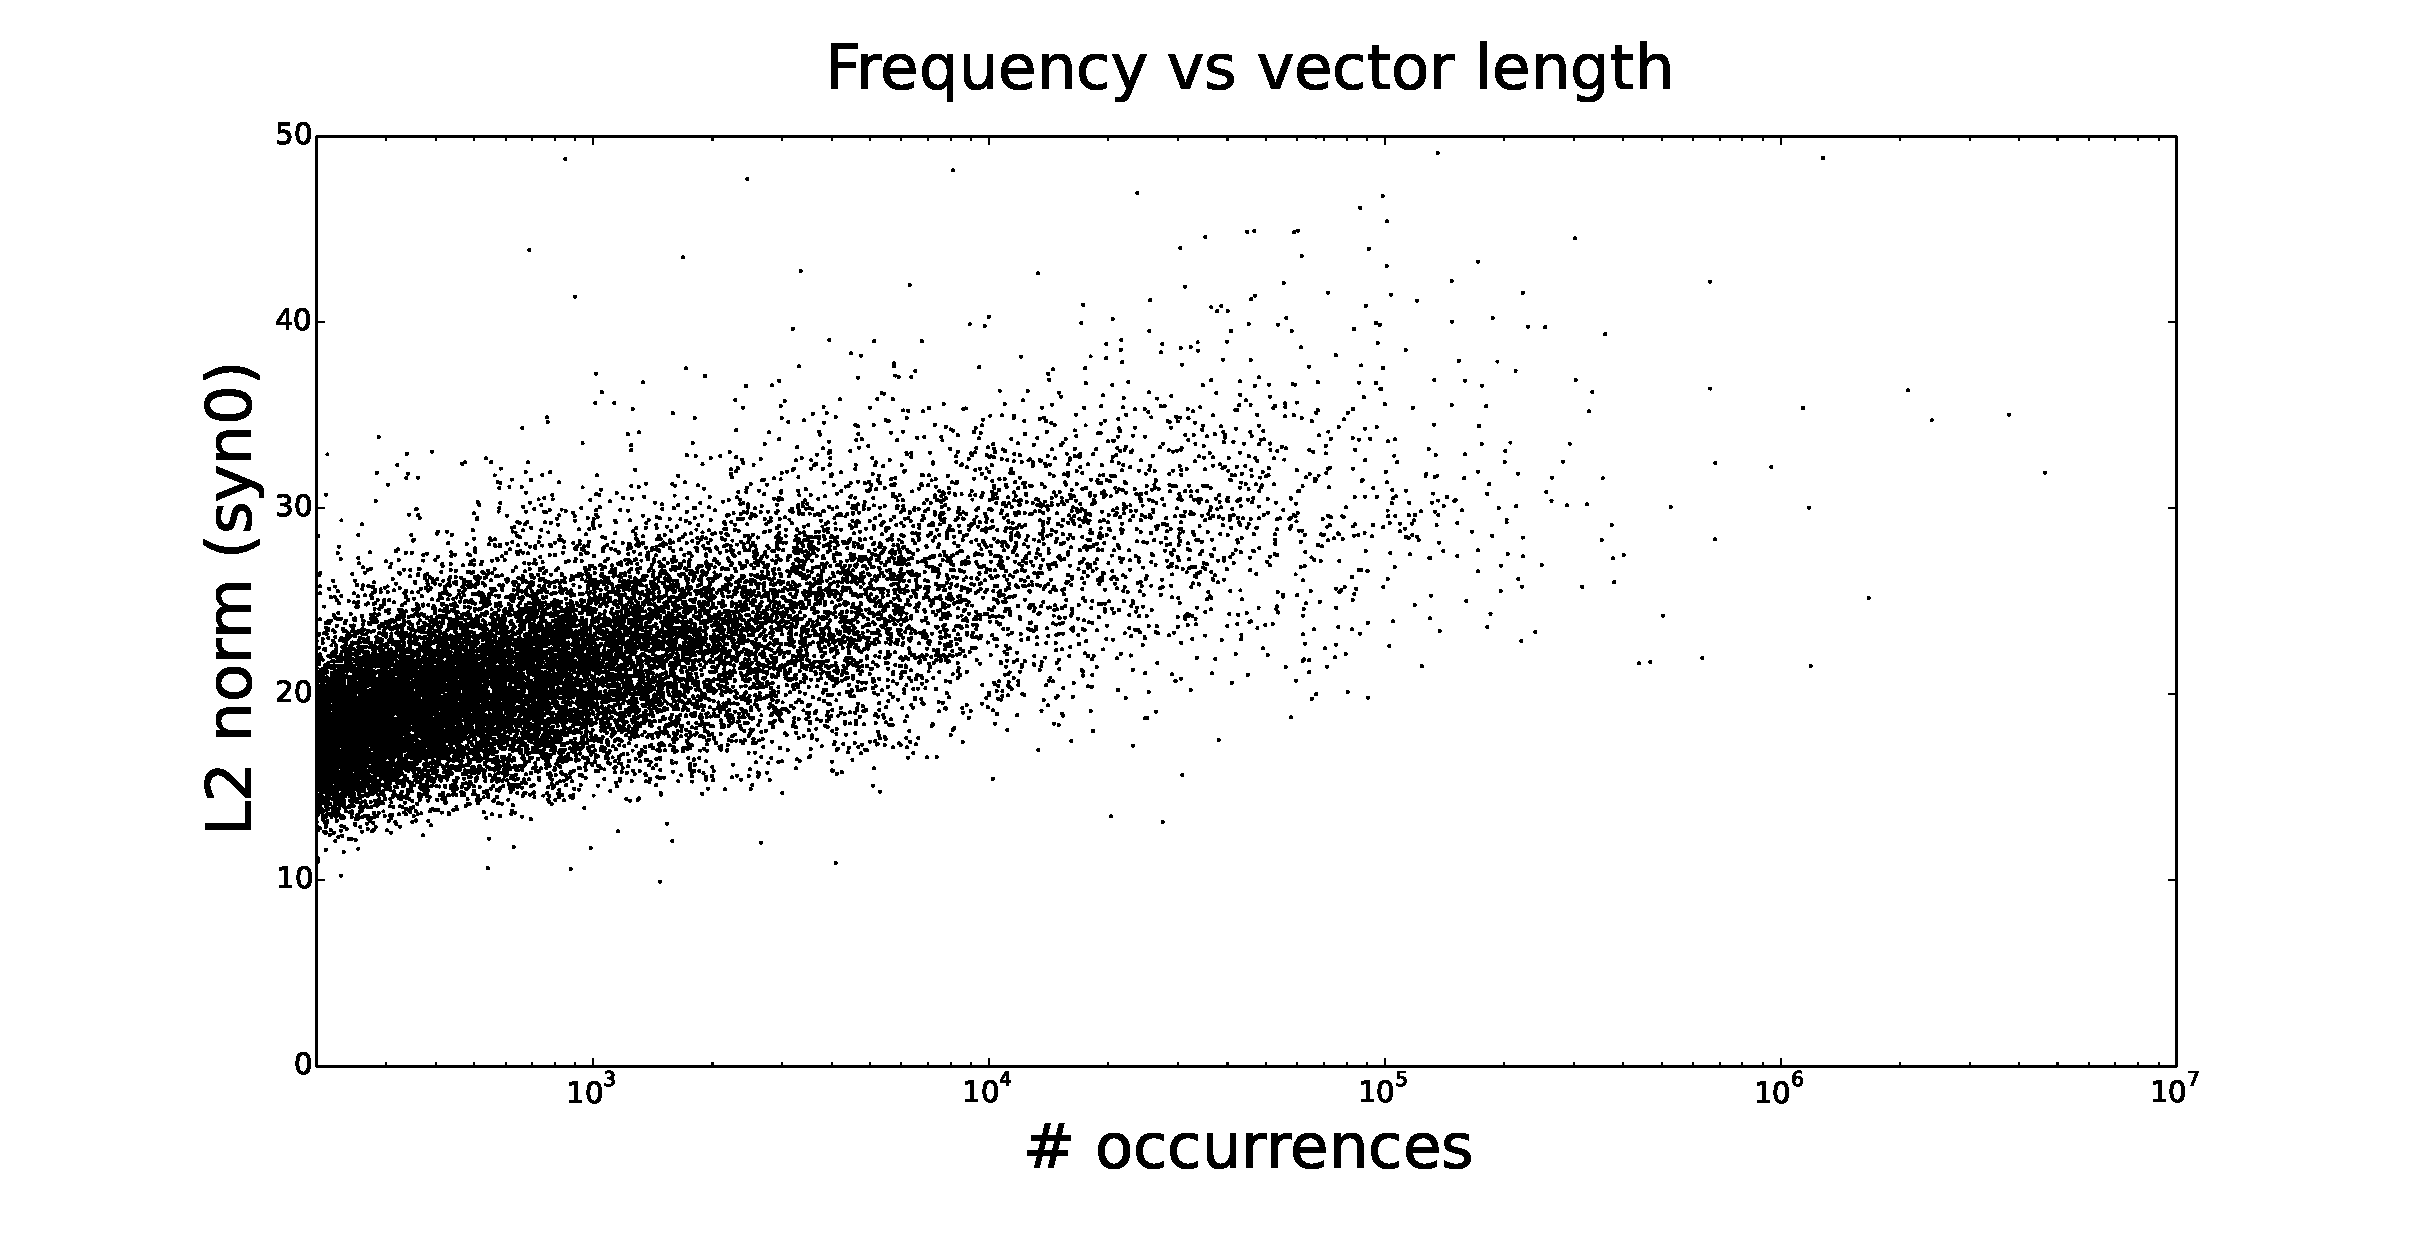
\includegraphics[scale=0.3]{frequency-norm-scatterplot}
\caption{ The global relationship between word frequency and vector length.  }
\label{fig:frequency-norm-graph}
\end{figure*}

\begin{figure*}
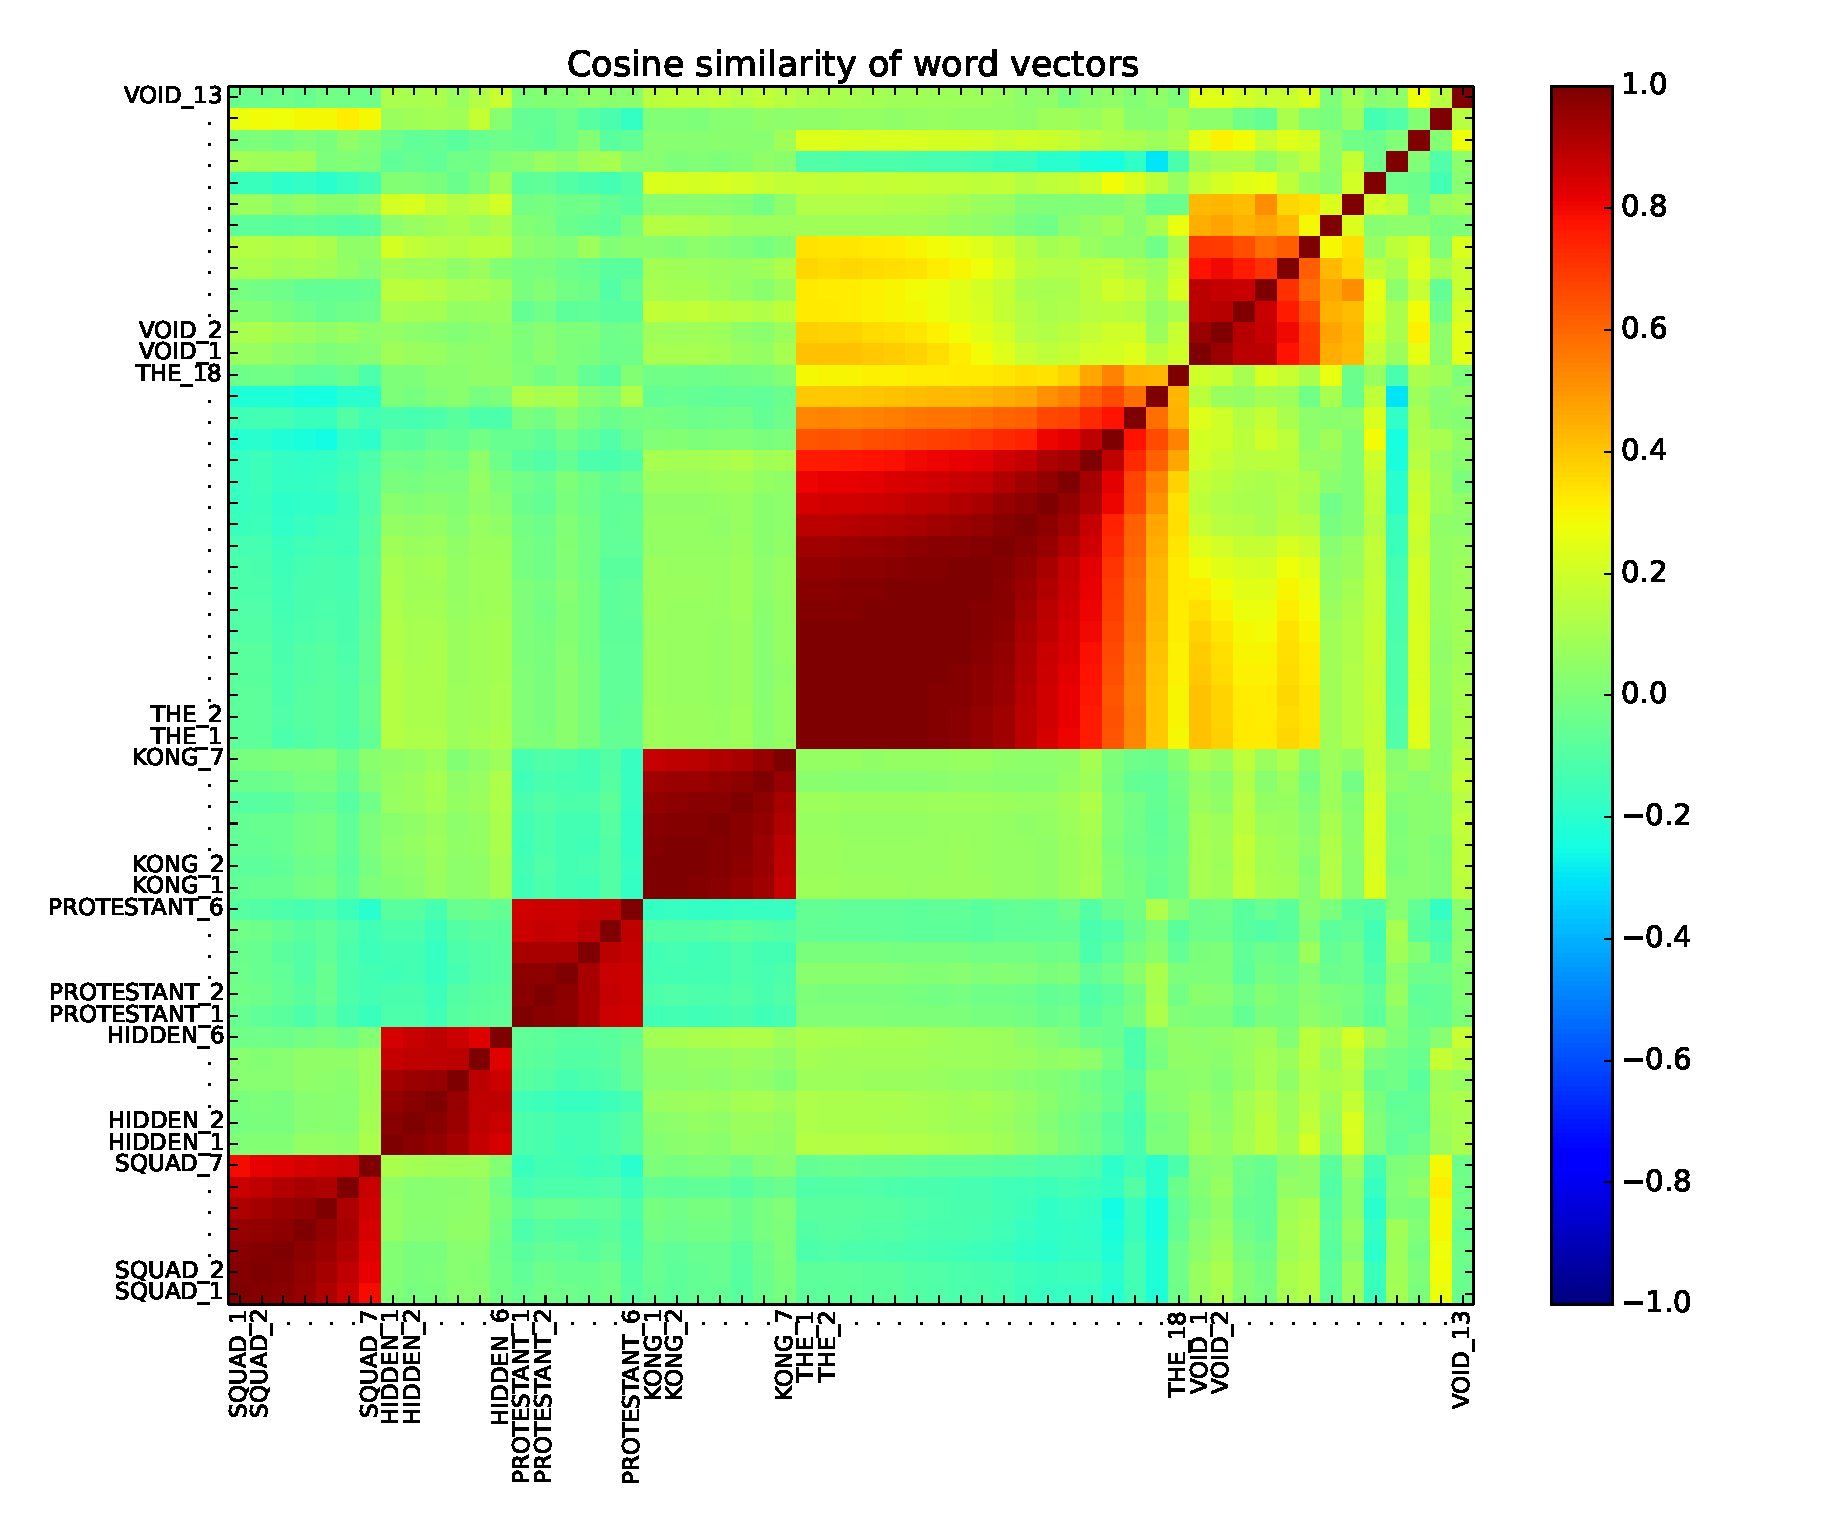
\includegraphics[scale=0.5]{word-frequency-experiment-heatmap}
\caption{
Heatmap of the dot product of the normalised vectors associated to the tokens introduced into the corpus in the co-occurrence noise experiment (four such words chosen at random).
The largely red blocks demonstrate that the direction of the word vector does not change when noise is added to the co-occurrence distribution.
}

\label{fig:cooccurrence-noise-heatmap}
\end{figure*}
\begin{sidewaysfigure*}
	\centering{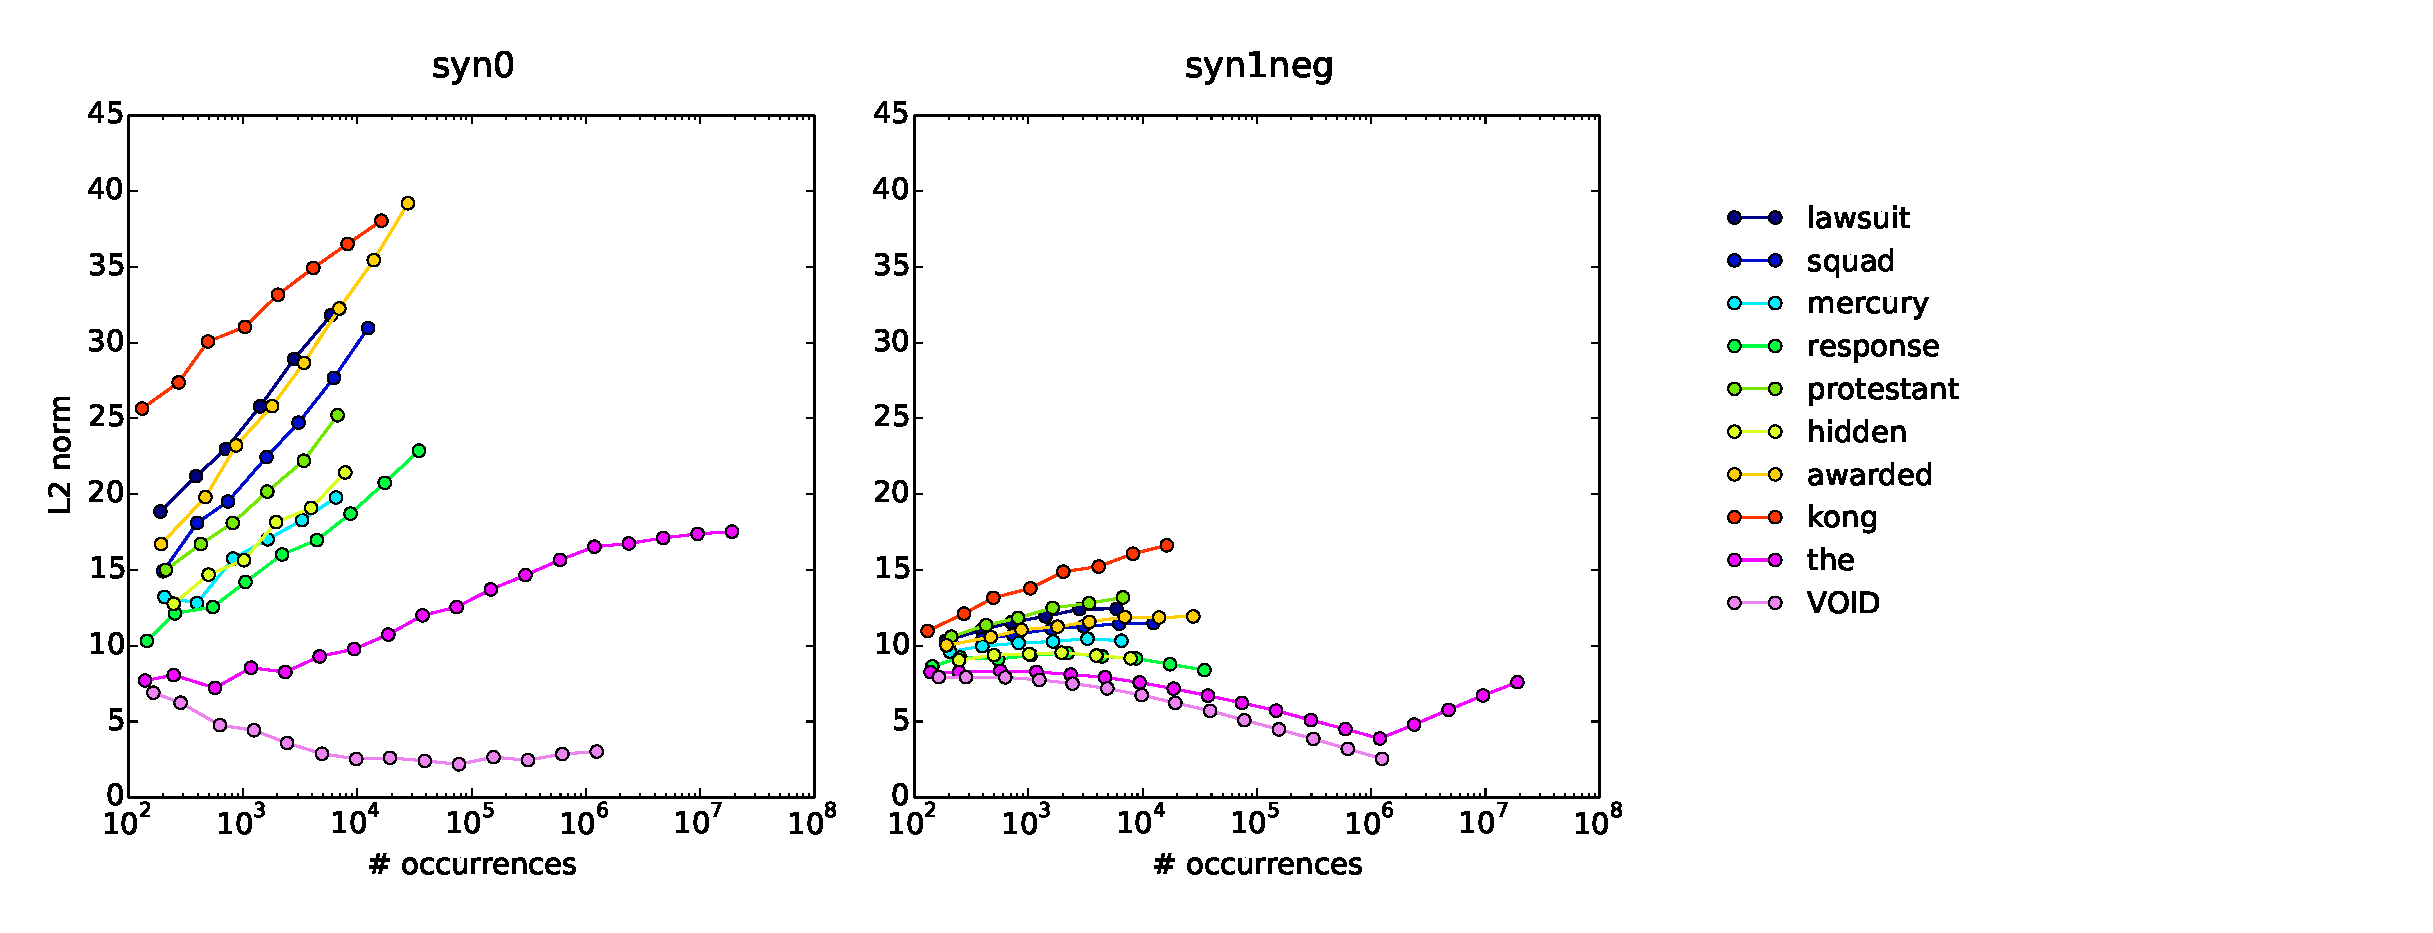
\includegraphics[scale=0.6]{word-frequency-experiment-graph}}
\caption{
	Vector length vs. frequency for the words chosen for the word frequency experiment.
	For each word, tokens of varying frequency but with the co-occurrence distribution of that word were introduced into the corpus, as described in section \ref{WFVE}.
}
\label{fig:word-frequency-experiment-graph}
\end{sidewaysfigure*}

\subsection{Co-occurrence noise experiment}
Consider the effect on a word vector when increasing levels of noise added to the co-occurrence distribution of the word.
This is affected by randomly dispersing an increasing proporition $0 \leqslant p \leqslant 1$ of the pre-existing occurrences of that word throughout the corpus.
The word vector depends on $p$, and thus $p$ parameterises a path in the feature space.
This path begins (with $p=0$) at the original word vector, and ends (with $p=1$) at the vector associated with the meaningless vector \word{VOID}.

For each word (e.g. \word{jury}) in the co-occurrence noise experiment, the vectors associated with the tokens \word{JURY\_i} mark points along this word's path for increasing values of $p$.
Figure \ref{fig:cooccurrence-noise-heatmap} shows that these points at all co-linear.
Thus the path is a straight line.

Figure \ref{fig:cooccurrence-noise-graph} illustrates the relationship between the proportion $p$ of co-occurrence noise and vector length.
Remarkably, it is apparent that this relationship is linear for any individual word.
Thus the norm decreases at a constant velocity as $p$ travels from $0$ to $1$.

It is Figure \ref{fig:cooccurrence-noise-graph} that motivates the interpretation of vector length, within a sufficiently frequency band, as a measure of the absence of co-occurrence noise, that is, of the extent to which a word determines a context.

\begin{sidewaysfigure*}
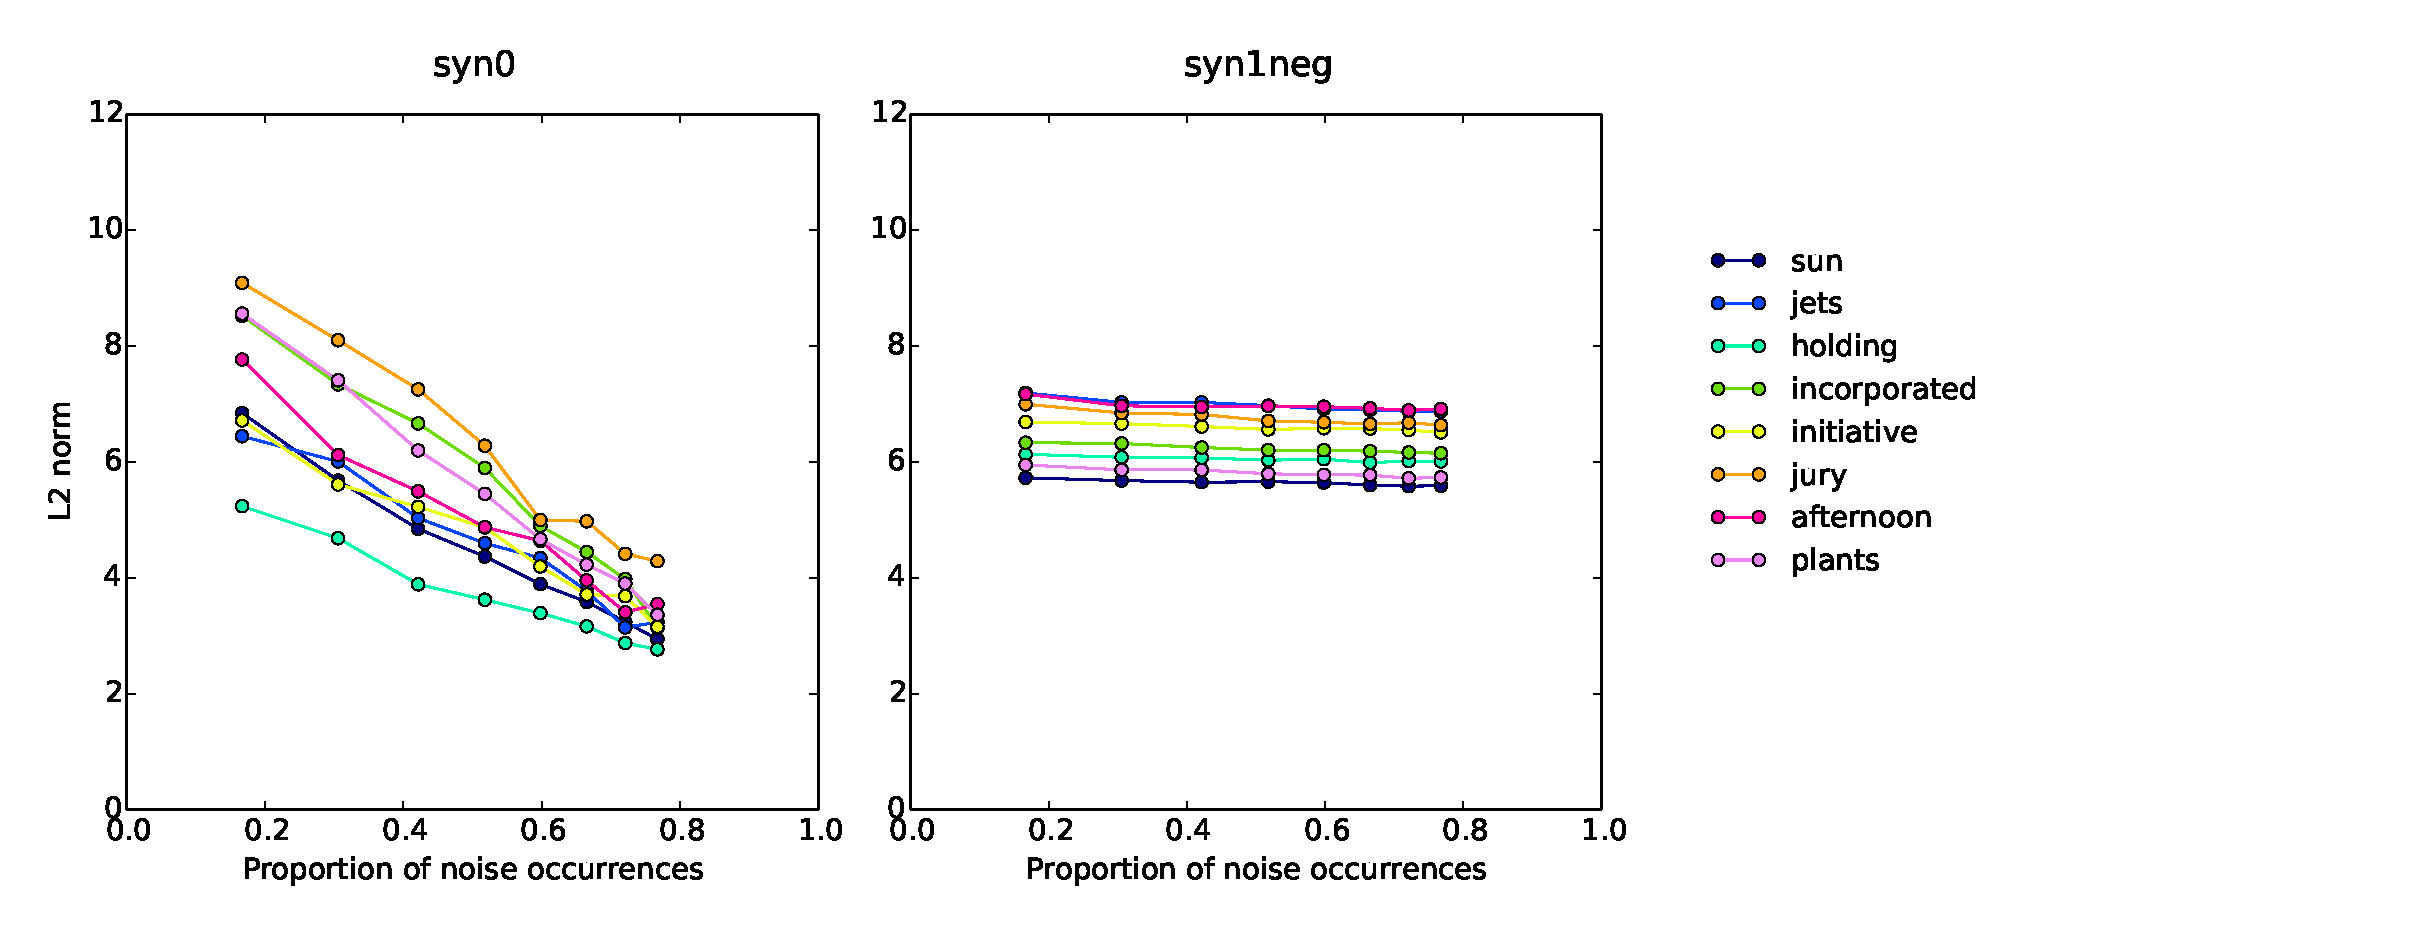
\includegraphics[scale=0.6]{cooccurrence-noise-graph}
\caption{
	Vector length vs. proportion of co-occurrence noise for words chosen for the co-occurrence noise experiment.
	For each word, tokens of equal frequency but with increasing proporitions of co-occurrence noise were introduced into the corpus, as described in subsection \ref{CNVE}.
}
\label{fig:cooccurrence-noise-graph}
\end{sidewaysfigure*}

\begin{figure*}[t!]
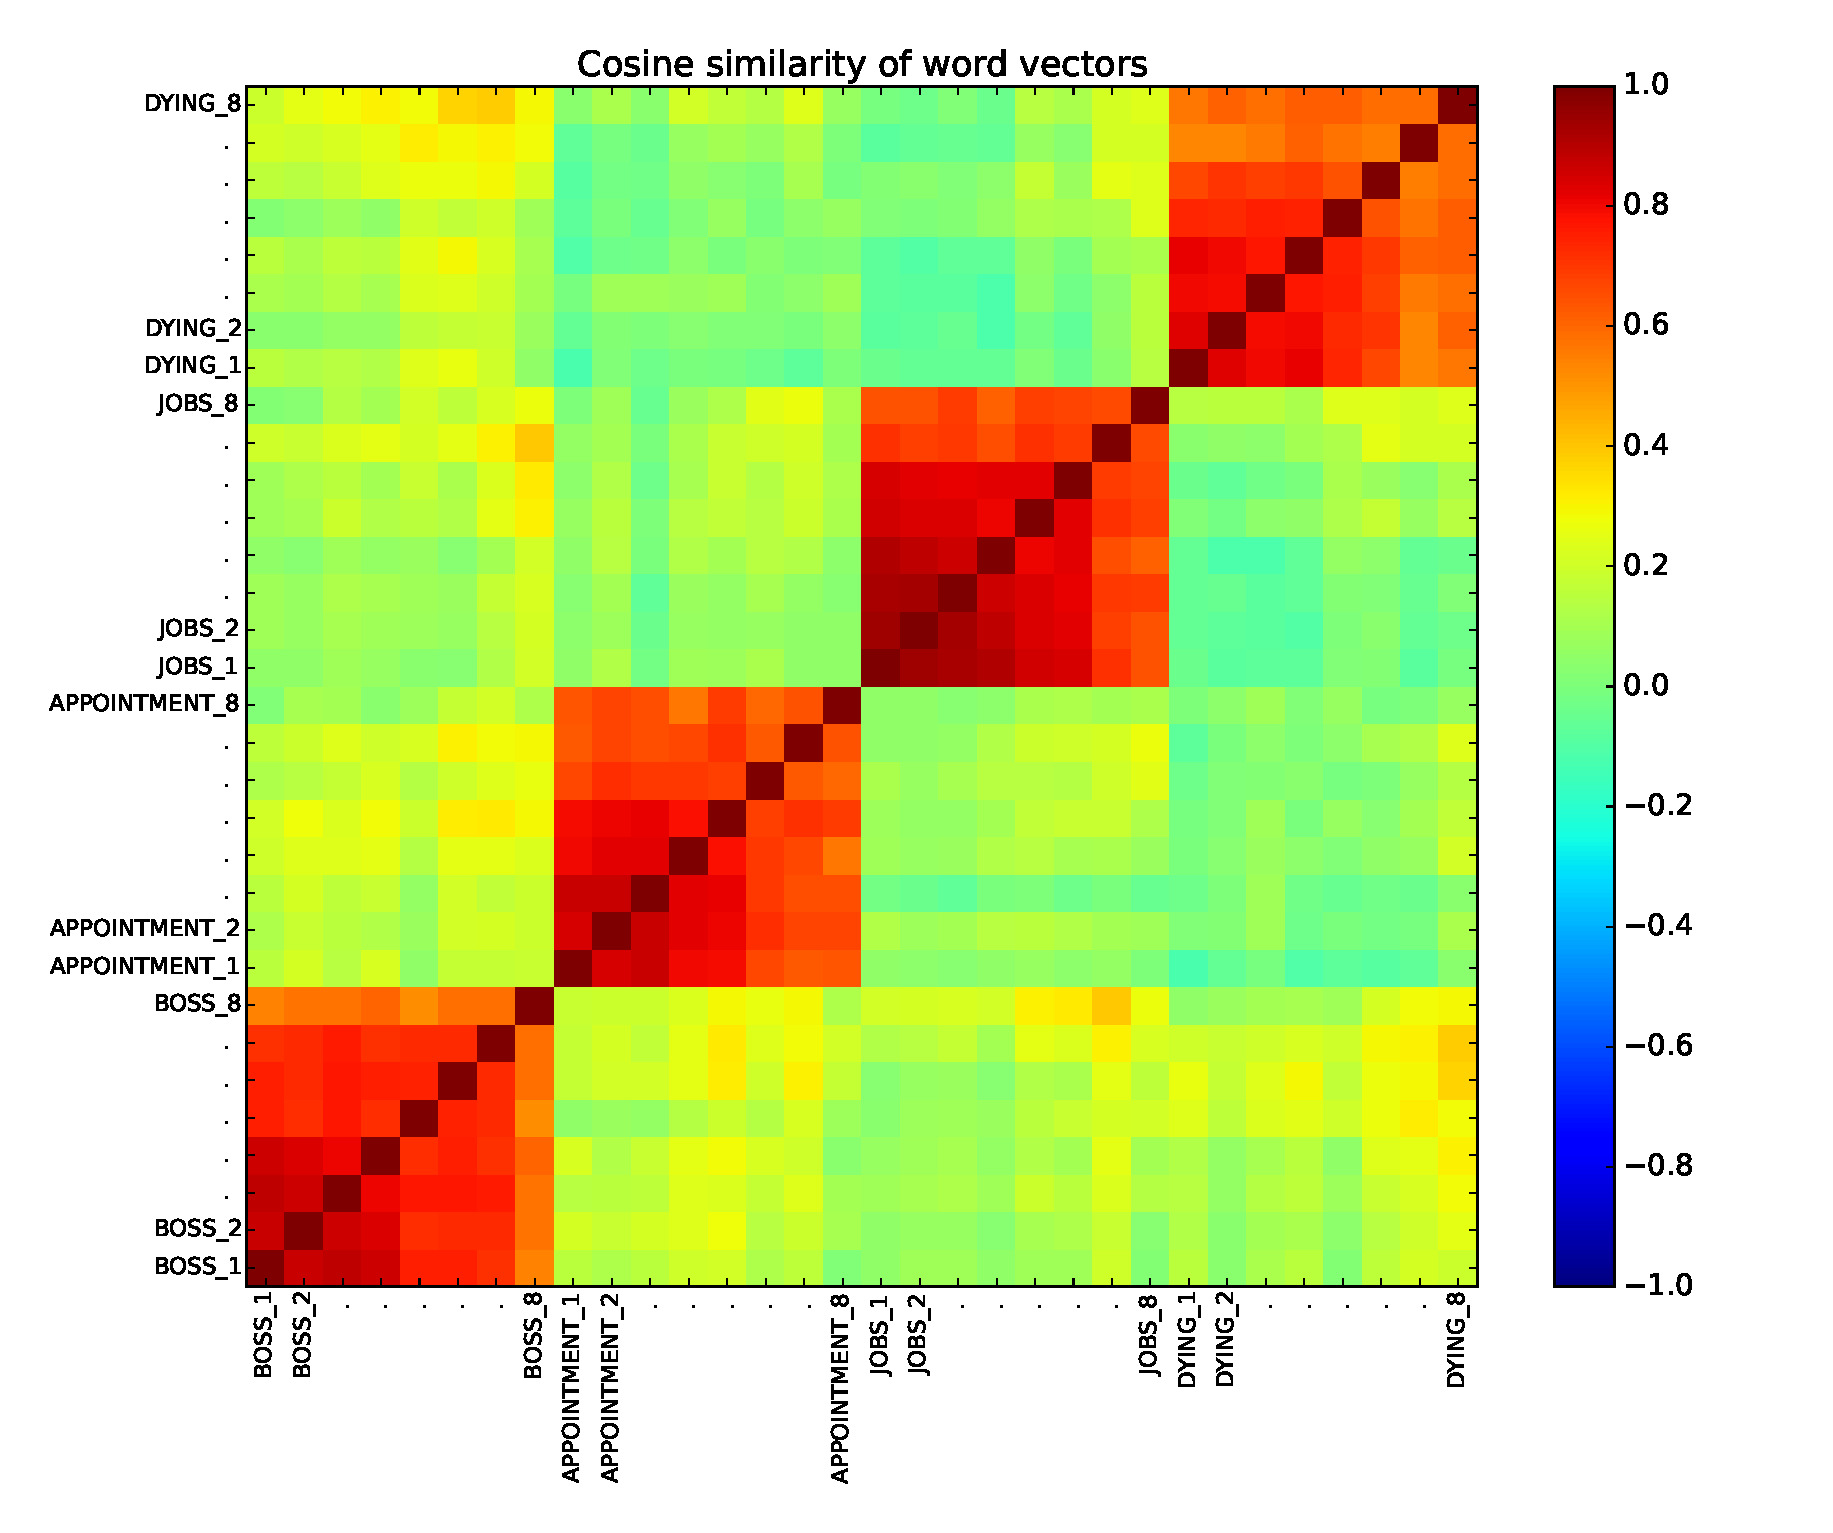
\includegraphics[scale=0.5]{cooccurrence-noise-heatmap}
\caption{
Heatmap of the dot product of the normalised vectors associated to the tokens introduced into the corpus in the co-occurrence noise experiment (four such words chosen at random).
The largely red blocks demonstrate that the direction of the word vector does not change when noise is added to the co-occurrence distribution.
}
\label{fig:cooccurrence-noise-heatmap}
\end{figure*}

\section{Questions}
\begin{enumerate}
\item{ Why is the meaningless vector not at zero, and could the performance on the compositionality tasks be improved by accounting for this?  Notice that the meaningless vector is only updated as part of the context vector.  Would it be zero if we were performing skipgram? Does this have something to do with the lack of bias terms in the word2vec softmax?}
\item{Our arguments from the results subsection on the co-occurrence noise experiment indicate that the meaningless vector should indeed be taken as the centre of the space for word similarity tasks.  Check again whether this works experimentally.}
\item{What is the distribution of norms for the vectors relative to the meaningless vector?  Do I need to consider a different meaningless vector for each frequency band?  This is the measure that should represent meaning.}

\end{enumerate}

\footnotesize
\bibliographystyle{unsrt}
\bibliography{main}

\end{document}
